\chapter{formulation of quantum statistics}
\section{quantum mechanical ensemble theory: the density matrix}
\begin{itemize}
	\item 用 density matrix 描述一个 ensemble,
	\begin{equation}
		\rho = \sum_i p_i \ket{\psi_i} \bra{\psi_i},
	\end{equation}
	在 Schrödinger 绘景下
	\begin{equation}
		i \hbar \frac{\partial \rho}{\partial t} = [H, \rho].
	\end{equation}
	\begin{itemize}
		\item density matrix 满足
		\begin{equation}
			\mathrm{Tr} \, \rho = 1, \quad \mathrm{Tr} \, \rho^2 \leq 1,
		\end{equation}
		其中第二个等号在 pure state 下成立.
	\end{itemize}
	
	\item the von Neumann entropy is
	\begin{equation}
		S = - \mathrm{Tr} \, \rho \ln \rho.
	\end{equation}
	
	\item stationary ensemble 的定义与 chapter \ref{2} 中一样, 见 \eqref{2.1.2}.
\end{itemize}

\section{statistics of the various ensembles}
\subsection{the microcanonical ensemble}
\begin{itemize}
	\item microcanonical ensemble 的 density matrix 为
	\begin{equation}
		\rho = \sum_{\text{some} \ i} \frac{1}{\Omega} \ket{i} \bra{i},
	\end{equation}
	其中 $\ket{i}$ 是能量本征态, 对所有 accessible states 求和.
\end{itemize}

\subsection{the canonical ensemble}
\begin{itemize}
	\item canonical ensemble 的 density matrix 为
	\begin{equation}
		\rho = \frac{e^{- \beta H}}{Z_\text{C}}, \quad Z_\text{C} = \mathrm{Tr} \, e^{- \beta H}.
	\end{equation}
	
	\item 各热力学量为
	\begin{equation}
		\begin{dcases}
			F = - k_B T \ln Z_\text{C}(T, V, N) \\
			S = - \Big( \frac{\partial F}{\partial T} \Big)_{V, N} = k_B \Big( \ln Z_\text{C} + T \frac{\partial}{\partial T} \ln Z_\text{C} \Big)
		\end{dcases}.
	\end{equation}
\end{itemize}

\subsection{the grand canonical ensemble}
\begin{itemize}
	\item grand canonical ensemble 的 density matrix 为
	\begin{equation}
		\rho = \frac{e^{- \beta (H - \mu N)}}{Z_\text{GC}}.
	\end{equation}
	
	\item 各热力学量为
	\begin{equation}
		\begin{dcases}
			\Phi_\text{G} = k_B T \ln Z_\text{GC}(T, V, \mu) \\
			S = \Big( \frac{\partial \Phi_\text{G}}{\partial T} \Big)_{V, \mu} = k_B \Big( \ln Z_\text{GC} + T \frac{\partial}{\partial T} \ln Z_\text{GC} \Big)
		\end{dcases}.
	\end{equation}
\end{itemize}

\section{example: an electron in a magnetic field}
\begin{itemize}
	\item 电子自旋为 $\frac{\hbar}{2} \vec{\sigma}$, 那么电子在磁场中的 Hamiltonian 为
	\begin{equation}
		\hat{H} = - \mu_0 (- \mu_B \vec{\sigma}) \cdot \vec{H} = \mu_0 \mu_B H \sigma_z,
	\end{equation}
	其中 Bohr magneton $\mu_B = \frac{e \hbar}{2 m}$.
	
	\item density matrix in the canonical ensemble is
	\begin{equation}
		\rho = \frac{e^{- \beta \hat{H}}}{Z_\text{C}} = \frac{1}{2 \cosh(\beta \mu_0 \mu_B H)} \begin{pmatrix}
			e^{- \beta \mu_0 \mu_B H} & 0 \\
			0 & e^{\beta \mu_0 \mu_B H}
		\end{pmatrix}.
	\end{equation}
	
	\item 得到
	\begin{equation}
		\braket{\sigma_z} = \mathrm{Tr}(\sigma_z \rho) = \tanh(\beta \mu_0 \mu_B H).
	\end{equation}
\end{itemize}

\section{the thermal de Broglie wavelength and the statistical potential}
\begin{itemize}
	\item 考虑一个由 2 个 indistinguishable 粒子组成的系统.
	
	\item 在 $\vec{x}_1, \vec{x}_2$ 分别发现一个粒子的概率密度为
	\begin{equation} \label{5.4.1}
		\tensor[_{\text{F or B}}]{\braket{\vec{x}_1, \vec{x}_2 | \rho_\text{C} | \vec{x}_1, \vec{x}_2}}{_{\text{F or B}}} \approx \frac{1}{V^2} \Big( 1 + \eta e^{- 2 \pi \frac{|\vec{x}_1 - \vec{x}_2|^2}{\lambda^2}} \Big), \quad \eta = \begin{dcases}
			+ 1 & \text{Bosons} \\
			- 1 & \text{Fermions}
		\end{dcases},
	\end{equation}
	其中
	\begin{equation} \label{5.4.2}
		\lambda = \Big( \frac{2 \pi \beta \hbar^2}{m} \Big)^{\frac{1}{2}} = \frac{h}{\sqrt{2 \pi m k_B T}}
	\end{equation}
	称为 thermal de Broglie wavelength, 如果 $n \lambda^3 \ll 1$, 量子效应不明显, 可以使用 Boltzmann statistics.
	
	\begin{tcolorbox}[title=calculation:]
		\begin{align}
			\tensor[_{\text{F}}]{\braket{\vec{x}_1, \vec{x}_2 | e^{- \beta H} | \vec{x}_1, \vec{x}_2}}{_{\text{F}}} &= \int \frac{d^3 k_1}{(2 \pi)^3} \frac{d^3 k_2}{(2 \pi)^3} e^{- \beta \big( \frac{k_1^2}{2 m} + \frac{k_2^2}{2 m} \big)} \frac{1}{2} \Big( 1 - \mathrm{Re} \, e^{i (\vec{x}_1 - \vec{x}_2) \cdot (\vec{k}_1 - \vec{k}_2)} \Big) \notag \\
			&= \frac{1}{2} \frac{1}{(2 \pi)^6} \Big( \frac{2 \pi m}{\beta \hbar^2} \Big)^3 - \frac{1}{2} \frac{1}{(2 \pi)^6} \Big( \frac{2 \pi m}{\beta \hbar^2} \Big)^3 \mathrm{Re} \, \exp \Big( - \frac{m}{\beta \hbar^2} |\vec{x}_1 - \vec{x}_2|^2 \Big) \notag \\
			&= \frac{1}{2 \lambda^6} \Big( 1 - e^{- 2 \pi \frac{|\vec{x}_1 - \vec{x}_2|^2}{\lambda^2}} \Big),
		\end{align}
		那么
		\begin{align}
			Z_\text{C} &= \int d^3 x_1 d^3 x_2 \, \tensor[_{\text{F}}]{\braket{\vec{x}_1, \vec{x}_2 | e^{- \beta H} | \vec{x}_1, \vec{x}_2}}{_{\text{F}}} \notag \\
			&= \frac{V^2}{2 \lambda^6} - \frac{1}{2 \lambda^6} \int d^3 x_1 d^3 x_2 \, e^{- 2 \pi \frac{|\vec{x}_1|^2 + |\vec{x}_2|^2 - 2 \vec{x}_1 \cdot \vec{x}_2}{\lambda^2}} \notag \\
			&= \frac{V^2}{2 \lambda^6} - \frac{1}{2 \lambda^6} \int d^3 x_2 \, e^{- 2 \pi \frac{|\vec{x}_2|^2}{\lambda^2}} \Big( \frac{\pi \lambda^2}{2 \pi} \Big)^{\frac{3}{2}} e^{\frac{\lambda^2}{8 \pi} \big( \frac{4 \pi}{\lambda^2} \vec{x}_2 \big)^2} \notag \\
			&= \frac{V^2}{2 \lambda^6} \Big( 1 - \frac{1}{2^{3 / 2}} \frac{\lambda^3}{V} \Big) \approx \frac{V^2}{2 \lambda^6},
		\end{align}
		Bosons 的情况类似.
	\end{tcolorbox}
	
	\item 如果两个粒子可区分,
	\begin{equation}
		\braket{\vec{x}_1, \vec{x}_2 | \rho_\text{C} | \vec{x}_1, \vec{x}_2} = \frac{1}{V^2}.
	\end{equation}
	
	\item 因此, \eqref{5.4.1} 中的 correlation 可以用一个势能 $v_s(r)$ 替代, 从而用经典力学的方法模拟这种量子统计效应,
	\begin{equation}
		v_s(r) = - k_B T \ln \Big( 1 + \eta e^{- 2 \pi \frac{|\vec{x}_1 - \vec{x}_2|^2}{\lambda^2}} \Big),
	\end{equation}
	函数图像如下:
	
	\begin{figure}[H]
		\centering
		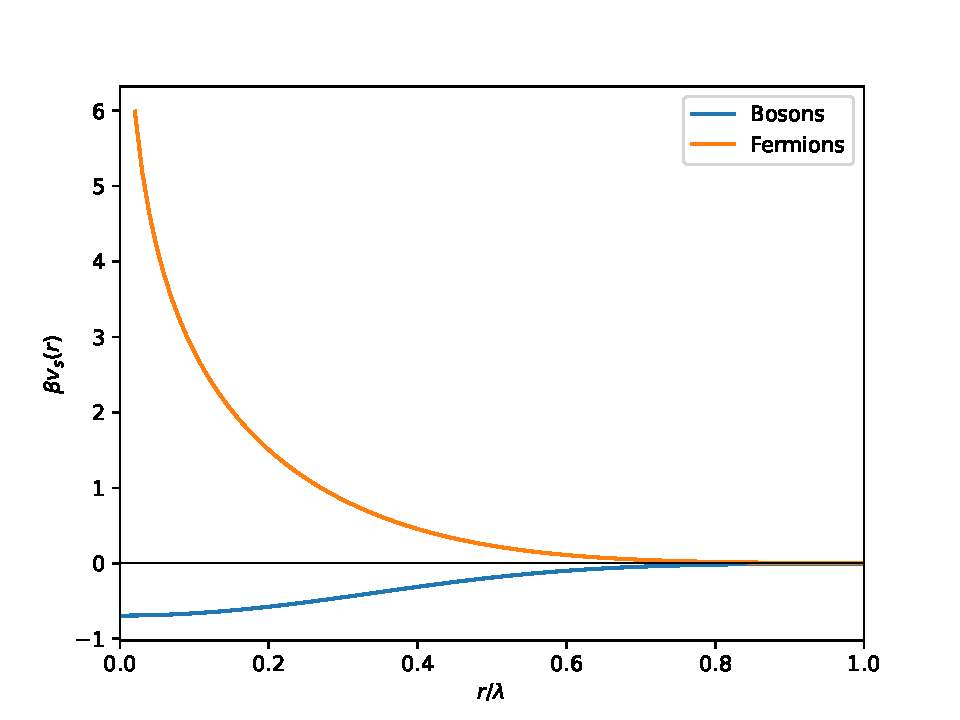
\includegraphics[scale=0.5]{figures/statistical potential.pdf}
		\caption{statistical potential.}
	\end{figure}
	
	\begin{tcolorbox}[title=proof:]
		只需要在 canonical ensemble 中引入一个 Boltzmann factor
		\begin{equation}
			e^{- \beta v_s(r)} = 1 + \eta e^{- 2 \pi \frac{|\vec{x}_1 - \vec{x}_2|^2}{\lambda^2}}.
		\end{equation}
	\end{tcolorbox}
\end{itemize}

\section{eigenstate thermalization hypothesis}
\begin{itemize}
	\item ergodicity of classical systems 要求几乎所有初始态都演化到均匀覆盖相空间中的等能面.
	\begin{itemize}
		\item integrable systems 一定不是 ergodic, 因为它们有 $\nu$ 个 constants of motion, 无法覆盖 $\nu - 1$ 维 energy surface.
		
		\item ergodic hypothesis 只在几个特例里被证明, 如 hard sphere gas.
	\end{itemize}
	
	\item 因为量子系统的演化有幺正性, 所以即便对应的经典系统有遍历性, 这个量子系统也不可能出现 ergodic-like behavior, 因此孤立的量子系统不可能热化.
	
	\noindent\hdashrule[0.5ex]{\linewidth}{0.5pt}{1mm} % horizontal dashed line
	
	\item 如果一个可观测量 $\braket{O}$ 从 a wide range of possible initial values, 在实验时间尺度内, 演化到一个 unique time-independent value (with small fluctuations), 则称 $O$ 表现出 equilibrium behavior,
	\begin{equation}
		O \ \text{displays equilibrium behavior} \iff \lim_{t \rightarrow \infty} \braket{O(t)} = \text{Const.}.
	\end{equation}
	\begin{itemize}
		\item 一般来说, 这样的 $O$ 不可能存在, 因为
		\begin{equation}
			\braket{\psi(t) | O | \psi(t)} = \sum_{m, n} c_m^* O_{m n} c_n e^{- i (E_n - E_m) t / \hbar},
		\end{equation}
		其时间平均值为
		\begin{equation}
			\text{time average of} \ \braket{O(t)} = \sum_n |c_n|^2 O_{n n} + \sum_{E_m = E_n, m \neq n} c_m^* O_{m n} c_n,
		\end{equation}
		永远依赖于初始条件.
	\end{itemize}
	
	\noindent\rule[0.5ex]{\linewidth}{0.5pt} % horizontal line
	
	\item 但是, 可能存在一些多体系统, 它们的  a large but restricted set of pure states and a large but restricted set of observables will thermalize.
	
	\item 注意到:
	\begin{itemize}
		\item 对于 homogeneous systems, $S \propto \nu$, ($\nu$ 是 degrees of freedom), 因此能量本征态的数量正比于 $e^{\alpha \nu}$.
		
		\item 能级简并数可以忽略, (比如理想气体 $\Omega(E) \propto \big( \frac{e^{\alpha'}}{\nu} \big)^\nu$).
	\end{itemize}
	
	\item 此时
	\begin{equation}
		\text{time average of} \ \braket{O(t)} \simeq \sum_n |c_n|^2 O_{n n},
	\end{equation}
	考虑 pure state with energy eigenvalue $E$,
	\begin{equation}
		c_n \neq 0 \quad \text{when} \quad E_n = E,
	\end{equation}
	令
	\begin{equation}
		O_{n n} = O(E) + \delta O_n, \quad E_n = E,
	\end{equation}
	且如果 $\delta O_n$ 满足
	\begin{equation}
		\sum_n |c_n|^2 \delta O_n \ll O(E), \forall c_n,
	\end{equation}
	那么 $\braket{O(t)}$ 的时间平均就与初始条件 (即 $c_n$) 的选取无关了.
	
	\item 最后, 还要求 $\braket{O(t = 0)}$ 可以明显偏离 $O(E)$, 但是随后 $t > 0$ 时的涨落却可以忽略.
	
	\noindent\hdashrule[0.5ex]{\linewidth}{0.5pt}{1mm} % horizontal dashed line
	
	\item 满足这些条件的 local operator 具有如下形式
	\begin{equation}
		O_{m n} \approx O(E_n) \delta_{m n} + \frac{O_2(E_m, E_n)}{\sqrt{\Gamma}} R_{m n},
	\end{equation}
	其中 $\{R_{m n}\}$ 是一个 $\Gamma \times \Gamma$ real symmetric Gaussian random matrix, $O(\cdot), O_2(\cdot, \cdot)$ 是光滑函数.
	
	\item random matrix $R$ 具有以下特征:
	\begin{itemize}
		\item 对角元平均值为 $0$, and variance $\sigma^2 = 2$.
		
		\item 满足
		\begin{equation} \label{5.5.9}
			\begin{dcases}
				\frac{1}{\Gamma} \braket{\mathrm{Tr} \, R} = 0 \\
				\frac{1}{\Gamma} \braket{\mathrm{Tr} \, R^2} = \Gamma + 1
			\end{dcases},
		\end{equation}
		其中 $\braket{\cdot}$ 表示对矩阵元的 normal distribution 的期望值.
		
		\item 对于 $\Gamma \gg 1$, $R$ 的本征值 $\lambda$ 的概率分布函数呈半圆形
		\begin{equation}
			\rho(x = {\textstyle \frac{\lambda}{\sqrt{\Gamma}}}) = \frac{1}{2 \pi} \sqrt{4 - x^2}, x \in [- 2, 2],
		\end{equation}
		因此 $\braket{(\Delta \lambda)^2} = \Gamma$, 与 \eqref{5.5.9} 相符 ($\Gamma \gg 1$).
		
		\item 还有一些性质, 见 Pathria, Beale, \textit{Statistical Mechanics}, page 147.
	\end{itemize}
	
	\item ...
\end{itemize}
